\documentclass[11pt]{article}

\usepackage{algorithm2e}
\usepackage{algorithmic} 
\usepackage{amsmath}
\usepackage{amsthm}
\usepackage{booktabs}
\usepackage{dcolumn} 
\usepackage{epstopdf}
\usepackage{fourier}
\usepackage{fullpage}
\usepackage{graphicx}
\usepackage{hyperref}
\usepackage{longtable} 
\usepackage{natbib}
\usepackage{rotating}
\usepackage{tabularx}

\hypersetup{
  colorlinks = TRUE,
  citecolor=blue,
  linkcolor=red,
  urlcolor=black
}

\begin{document} 

\newtheorem{prop}{Proposition}


%\title{Peer-to-Peer Computer-Mediated Rental Markets: \\ A Model of Collaborative Consumption}
%\title{Consumers Renting Their Goods to Other Consumers}
%\title{The Introduction of Rental Markets in Consumer Goods} 
%\title{Buy, Buy and Rent Out, or Rent? \\ Consumer Theory in the Presence of Peer-to-Peer Rental}
%\title{Peer-to-Peer Rental Markets}  
\title{The Simple Economics of the So-Called Sharing Economy} 

\date{\today}

\author{John J. Horton \\ Leonard N. Stern School of Business \\ New York University\footnote{ Author contact information, datasets and code are currently or will be available at \href{http://www.john-joseph-horton.com/}{http://www.john-joseph-horton.com/}. } }
\maketitle

\begin{abstract}
\noindent  I consider a model where the owners of goods can use those capital goods themselves and, at some cost, rent them in a marketplace. 
What goods are likely to be shared. 
What are the welfare consequences. 
Will overall product demand go up or down? \newline
\noindent JEL J01, J24, J3
\end{abstract} 


% http://www.forbes.com/pictures/ehfk45edlgh/0122_sharing-williams-snapgoods_650x455-jpg/
% http://www.zdnet.com/the-sharing-economy-that-doesnt-exist-7000030137/
% http://www.economist.com/news/leaders/21601257-too-many-obstacles-are-being-placed-path-people-renting-things-each-other-remove
% http://meshing.it/
% These cites have lowered the opportunity cost r
% http://petapixel.com/2013/07/16/camera-gear-rentals-is-big-business-and-lensrentals-proves-it/ 
% www.salon.com/2013/09/17/the_sharing_economy_muscles_up/
% http://techcrunch.com/2012/02/27/following-thefts-luxury-car-sharing-service-higear-acquired-by-rent2buy/
% http://poshmarkapp.tumblr.com/post/73422383633/poshmark-s-closet-sharing-economy-report 
% http://www.forbes.com/sites/tomiogeron/2013/01/23/airbnb-and-the-unstoppable-rise-of-the-share-economy/

% Popular Books
% http://www.amazon.com/Mesh-Why-Future-Business-Sharing/dp/B00A16VVX8
% % http://www.amazon.com/Whats-Mine-Yours-Collaborative-Consumption/dp/0061963542/ref=pd_cp_b_0 

% From the Forbes article: 
% ``Additionally, GM can incentivize sales by promoting the idea that a new car can now come with a rental income stream attached.'' 


% “We’re going to have to invent new economics to capture the impact of the sharing economy,” says Arun Sundararajan, a professor at the Stern School of Business at NYU who studies this phenomenon. The largest question for academics is whether this all creates new value or just replaces existing businesses.

\section{Introduction}
Entrepreneurs are creating computer-mediated peer-to-peer rental markets for goods such as cars, clothing, tools, bicycles, camera equipment, apartments, offices, parking spaces and so on.
These marketplaces lower the transaction costs and informational problems that presumably made these kinds of peer-to-peer transactions previously uneconomical.
Perhaps the most prominent example is Airbnb, which allows individuals to rent out spare bedrooms, apartments or even entire homes: Airbnb was recently valued at TK and now has more stock of rooms than the TK hotel chain. 
 
This phenomena---sometimes called ``collaborative consumption'' and the broader development the ``sharing economy'' has attracted much business and policy interest.  
Proponents argue it lets owners put otherwise idle goods into use and expand access for people who could not or would not buy. 
Critics charge that their primary competitive advantage of these peer-to-peer lenders is regulatory arbitrage: 
not subject to the same regulations as conventional firms, P2P rentals are artificially (and inefficiently) cheap. 

Both proponents and critics are making implicit, albeit informal arguments about the economic nature of these markets.  
The purpose of this paper is to introduce a model of P2P rental of goods and explore its implications.  
Although rental markets have long-existed, the widespread renting by consumers to other consumers is something fundamentally new that requires an explanation.  
It also seeks to more formally characterize what makes a good ``rentable.'' 
First we consider an existing product market where consumers must decide whether or not to buy a good.
Consumers differ in their utility from using the good and those with relatively high expected use buy while those that do not go without.
Each consumer, regardless of the purchase price, has some optimal use fraction between 0 and 1, with 1 being use 100\% of the time (e.g., a heart pacemaker). 
We compare this purchase-only market to a pure rental market where the rental rate is the same as the purchase price. 


%% Car-sharing services like RelayRides, Uber, Sidecar and Lyft have repeatedly encountered regulatory resistance from nearly every city they have begun operations in, with that opposition often spearheaded by existing Taxi companies.   
%% Airbnb was---until recently---in a protracted fight with the New York Attorney General's office regarding hosts potential violation of New York City's illegal hotel laws.  
%% Further, critics argue that the renters in these markets are responding to harsh economic conditions and that they would not participate if there was a better economy. 

% \subsection{Ramesh Notes} 
% - Need to prove the uniqueness of equilibria 
% - How does depreciaation enter in? it's now a fixed cost for renters 
% - In the long-run, for the same market price p, the product market demand is less elastic because the marginal buyer can not receive rental income, which rises with the product market price. It's not completely offsetting, 
% - If product market demand less elastic, if the products have market power product market prices should rise.  
% - To owners to fully internalize benefits?    

The general characteristic of goods that are ``rentable'' are those that are used infrequently but are expensive: 
cars and hotels in distant cities, tuxedos, certain tools, etc.
However, these goods were usually offered by a company who owned the stock with the explicit purpose of renting.  
And although individuals are owned by at least some consumers who would have excess capacity, the transaction costs of facilitating peer-to-peer rentals would be prohibitive
Simply finding an appropriate trading partner would be difficult, to say nothing of coming to terms, writing a contract, monitoring compliance, handling disputes, making payment and so on. 
Further, those individuals that owned a good despite the existence of a rental market were likely those with relatively little excess capacity to rent out. 

A natural question is why these P2P markets are arising now? 
The short answer is that advances in information and communications technology are making them possible---particularly the mass adoption of the Internet and smart phones.  
Computer-mediated platforms can match supply and demand, nudge parties towards agreements, provide a regulatory and monitoring framework and take numerous steps to minimize adverse selection and moral hazard, such as maintaining a reputation system. 
As many of these services are offered algorithmically, the marginal cost of intermediation is close to zero, and by definition, capital costs are zero.  
The first effect of this development is to create rental markets where none existed before. 

\begin{table}
\caption{Sharing economy companies and the category of goods of services used}
\centering
\begin{tabular}{llc} 
\toprule
Good or Service & Company & Labor Component? \\ 
\hline Rooms           & Airbnb & No \\ 
Vacation homes  & VRBO   & No \\ 
Cars            & UberX, Lyft, RelayRides, Sidecar, Getaround & Yes \\   
Parking         & Park Circa, ParkatmyHouse, Parking Panda & No \\
Bicycles        & Liquid & No \\   
WiFi Router     & Fon & No \\ 
Boat            & Boatbound & No \\
Camera equipment& LensRentals & No \\  
Handman tools   & TaskRabbit  & Yes \\
Household goods & SnapGoods   & No \\ 
Kennel          & DogVacay   & Yes \\ 
Clothes         & GirlMeetsDress & No \\
\bottomrule
\end{tabular}  
\end{table}


\begin{table}
\caption{Research questions}
\centering
{\footnotesize 
\begin{tabular}{llp{8cm}} 
\toprule
Topic & Research Question & Model prediction \\ 
\hline 
{\bf Product market} \\ 
& What goods are amenable to sharing? & TK \\ 
& Effect of sharing on the product market price in the long-run & TK \\
& Long-run elasticity of demand & TK \\ 
& Why did the firm sell rather than rent? & TK \\    
{\bf Welfare} \\ 
& Prior-owners not renting out & TK \\ 
& Prior-owners now renting out & TK \\ 
& Prior non-owners now renting & TK \\
& Efficiency & TK \\ 
{\bf Rental rates} \\
& What is the short-run rental rate? & TK \\
& What is the long-run rental rate?  & TK \\ 
{\bf Participation} \\ 
& Who rents out in the long- and short-run? \\ 
{\bf Comparative statics---Transaction Costs} \\ 
& long-run rental rate & TK \\ 
& long-run product market price & TK \\ 
& Ownership shares & TK \\ 
\bottomrule
\end{tabular}  
}
\end{table}


There are several economic questions that this creation of peer-to-peer rentals raise. 
Does the product market demand for the durable good go up or down when P2P rental markets emerge?  
What determines the connection between the produce market price and rental rate in the long- and short-runs? 
How does the possibility of rental affect the elasticity of demand for the product? 
What are the welfare consequences for consumers? 
How does initial pattern of good ownership and how does it change? 
What goods are particularly amenable to sharing and why?  

To answer these questions, I develop a simple model that starts with a collection of would-be consumers for a good that make a purchasing decision before the possibility of rental.
Before the possibility of rental, some consumers buy a good and others do not, based on how intensively they plan to use the good after purchase and the indirect utility this provides.  
I then introduce the possibility that owners can rent to non-owners, creating a ``short run'' sharing economy. 
Next, I assume that all parties can adjust their buying and renting decisions, creating a ``long run'' which affects prices in the product market. 

I assume that this difference reflects differences in preferences, but not in a direct way, with some explicitly valuing the good more than others. 
Instead, I assume that consumers differ in their marginal utility from \emph{intensive} margin use of the good.
This can be thought of as what fraction of their time they spend using that good.  
Given these differences, conditional upon purchase, some consumers use the good very intensively (those with a high marginal utility from use) and some consumers would not use the good intensively. 
Consumers consider the indirect utility from their chosen level of intensive-margin consumption and compare it to the purchase price. 
Those whose indirect utility is greater buy the good, while those that do not go without.  
This creates a collection of owners, each of whom picks some level of usage. 

I assume that a technological shock creates the possibility of owners renting out their excess capacity to non-owners. 
There is a fixed cost to renting, which we might think of as the transaction cost plus the ``reset'' costs to counter any depreciation from more intensive use. 
With the possibility of renting, owners have to make two decisions: whether to rent at all given the rental rate and, when faced with a specific rental rate, how much to economize their own usage, which frees up supply to rent. 
Interestingly, those that rent and those that own and rent out face the same usage decision, the marginal cost of usage now includes the rental rate (for those that rent) and the foregone rental income (for those that own and rent out). 

For the short-run rental market to clear, the amount of supply from owners has to equal demand. 
This determines a rental rate, which is only indirectly related to the purchase price. 
In the long run, everyone is free to re-visit their ownership decision. 
If the short-run rental rate is below the purchase price plus the costs of renting, then ownership is less attractive, which will reduce \emph{purchase} demand for product, lowering prices. 
However, if the rental rate is above the purchase price plus the cost of renting, ownership becomes more attractive, increasing demand and raising purchase prices in the product market. 

Technological improvements that lower the costs of renting tend to bring more owner-provided supply of goods into the rental market, lowering rental rates. 
This in turn reduces the appeal of ownership, lowering prices in the product market. 
From the consumer perspective, reduced product market prices are Pareto improving regardless of whether the consumer rents, owns and rents out or owns but does not rent. 

Goods with high purchase prices but low and predictable intensive margin usage are ideal for P2P rental markets: 
the purchase price is high enough that there are lots of would-be consumers with high willingness to pay and enough owners with excess capacity that the market-clearing rental rate is not prohibitively high. 
When produce market prices are low, there is no excess demand so nearly everyone buys the product, so even if the good is used infrequently, no rental market can exist.  
For example, there is no rental market in kitchen timers or egg timers: although they are used very infrequently and quite durable, there is neither supply (no one owning finds it worth the trouble) nor demand (if one wants one, they go to the product market). 
Other goods are expensive but there is no excess capacity, as they are used more or less continuously. 
For example, there is no P2P rental market in heart pacemakers. 
There would also be no demand---if all owners want to use a good nearly 100\% of the time, then presumably so do would-be renters, and if that is true, they are not renters but rather owners, subject to budget constraints.   

\section{Nature of depreciation} 
Rental markets only exist for durable goods. 
For a P2P rental market to function, goods have to depreciate regardless of usage level. 
This makes it useful to use them up more quickly, through more intensive use. 

\section{Product market without rental} 
Consumers have a unit of time available and choose some fraction of their time, $x$ in $[0,1]$, to use the good. 
Consumers differ in their utility from usage: they get utility $\theta u(x)$ where $\theta \in [\underline{\theta}, \bar{\theta}]$, with $\theta \sim F$.  
Users pay a cost from usage of $cx$, where $c > 0$. 
I assume that $u'(x) > 0$ and $u''(x) < 0$ and $u(0) = 0$.
At a price $p$, a consumer buys the good if 
\begin{equation}
\theta u(x^*) - cx^* \ge p  
\end{equation} 
where $x^*$ maximizes the consumer's utility, conditional upon purchasing. 
Market demand for the product is 
\begin{equation}
D(p) = \int_{\theta_B}^{\bar{\theta}} f(\theta) \, d\theta  = 1 - F(\theta_B)
\end{equation} 
where $\theta_B$ is the $\theta$ of the consumer indifferent between buying and not buying. 
For the marginal buyer, $v(\theta_B) = 0$, where $v(\cdot)$ is the indirect utility function.  

\subsection{Elasticity of demand}
We can characterize the elasticity of demand based in part on the shape of $u()$ at $\theta_B$. 
The price elasticity of demand for the product is 
\begin{equation} 
E_D = \frac{D'(p)}{D(p)} = - \left(\frac{f(\theta_B)}{1-F(\theta_B)} \right) \frac{\partial \theta_B}{\partial p}. 
\end{equation} 
Using the first order condition and applying the envelope theorem, we have 
\begin{equation}
\frac{\partial \theta_B}{\partial p} = \frac{1}{u(x^*)} = \frac{\theta}{p + cx^*}. 
\end{equation} 
This implies that products with a lower $u(x^*(\theta_B))$ have more elastic demand.  
Consider Figure~\ref{fig:extensive_margin}, which shows the indirect utility function versus $\theta$ for two products. 
Note that both products have the same demand at price $p$ (same $\theta_B$). 
However, in the figure, the steeper slope comes from the product with the higher $u(x)$. 
Note that $\frac{\partial v}{\partial \theta} = u(x^*)$. 

\subsection{Comparative statics} 

\begin{prop}
An increase in $c$, the opportunity cost of time, lowers demand for the good.  
\end{prop} 
\begin{equation}
\frac{\partial x^*}{\partial c} = \frac{1}{\theta u''(x^*)} \le 0. 
\end{equation} 


\begin{figure}
\caption{Individual utility and demand on the extensive margin \label{fig:extensive_margin}} 
\centering 
\begin{minipage}{\textwidth} 
\includegraphics[width = 0.80 \linewidth]{./diagrams/extensive_margin_demand_elasticity.pdf}
{\footnotesize
\newline \emph{Notes:} This figure shows how different utility functions create different elasticities of demand on the extensive margin.  
}
\end{minipage}  
\end{figure} 

\section{Pure rental market} 
Initially, we assume that there is no friction. 
In this market, the quantify of the good consumed is just 
\begin{equation}
D(r) = \int_{\underline{\theta}}^{\bar{\theta}} x(\theta, c + r) d\theta,  
\end{equation} 
where $r$ is the rental rate. 
The chance in demand from a small increase in the rental rate is 
\begin{eqnarray*}
\frac{\partial D(r)}{\partial r} &=& \int_{\underline{\theta}}^{\bar{\theta}} \frac{\partial x(\theta, c + r)}{\partial r} d\theta  \\
                                 &=& \int_{\underline{\theta}}^{\bar{\theta}} \frac{1}{\theta u''(x)} d\theta  \\
                                 &=& \int_{\underline{\theta}}^{\bar{\theta}} \frac{1}{c+r}\frac{u'(x)}{\theta u''(x)} d\theta  \\
                                 &=& \frac{1}{c+r} \int_{\underline{\theta}}^{\bar{\theta}} \theta \frac{\partial x}{\partial \theta} d\theta  \\

\end{eqnarray*} 
and then, using integration by parts 
\begin{eqnarray}
\frac{\partial D(r)}{\partial r} &=& \frac{1}{c+r}\left[\bar{\theta}x(\bar{\theta}) - \int_{\underline{\theta}}^{\bar{\theta}} x(\theta) \right] \\ 
                                 &=& \frac{1}{c+r}\left[\bar{\theta}x(\bar{\theta}) - D(r) \right]
\end{eqnarray} 

How does a chance in $r$, the rental rate, affect demand? 


\section{A rental market with friction} 
When consumers faced a buy/no buy decision, all users with $\theta < \theta_B$ but with $\theta u'(0) > c$ wanted to consume some of the good but were unwilling to pay $p$ for it. 
Now we consider a frictionless rental market where $r = p$, meaning that the cost of fractional use ($x < 1$) is pro-rated proportionally to the product market price. 
Figure~\ref{fig:buy_versus_rent} shows the utility of buyers and renters versus $\theta$. 

At each value of $\theta$, conditional upon purchasing, a buyer uses the good more than a renter. 
The reason is that an owner's marginal opportunity cost is only $c$, whereas for a renter it is $c + r$. 
Since the slope of $\frac{\partial U}{\partial \theta} = u(x)$, and $u'(x) > 0$, the buyer curve as a higher consumption utility for all $\theta$ (though not a higher value function). 
Also, since $u(x)$ is increasing, both curves are convex (TK---not really shown). 

The first consumer that wants to rent has $\underline{\theta}_R = \frac{r + c}{u'(0)}$, whereas the first consumer that wants to buy has $\underline{\theta}_B = \frac{c}{u'(0)}$.

\begin{prop}
  The first ``renter'' at $\underline{\theta}_R$  will choose $x^* = 0$. 
\end{prop} 
\begin{proof}
For the first renter, $\theta u(x) - (c + r)x^* = 0$, and from the FOC, $\theta u'(x) = c + r$, which implies 
that $x^* u'(x^*) = u(x^*)$, but since $u(\cdot)$ is concave by assumption, $x^* = 0$.  
\end{proof} 

All buyers with $x^* < 1$ will strictly prefer to rent (and the buyer with $x = 1$ is indifferent). 
The reason is that for any consumer can consume the same amount as but at a lower cost, since $x^*r < p$. 
Consumers can do better under renting by economizing on their consumption of $x$ to reflect the new marginal cost of consumption, $c + r$. 
In this hypothetical friction-free rental market, consumer ownership disappears and all consumers rent. 
  
\begin{figure}
\caption{Indirect utilities of renting versus buying\label{fig:buy_versus_rent}} 
\centering 
\begin{minipage}{0.80 \textwidth} 
\includegraphics[width = \linewidth]{./diagrams/buy_versus_rent.pdf}
\end{minipage}  
\end{figure} 

Now we consider what happens when their is an additional cost to renting such that $r > p$.
This will create a $\hat{\theta}$ that divides consumers into buyers and renters. 
Those with $\theta > \hat{\theta}$---the heavy intensive-margin users---buy, whereas the more casual users rent. 
If $\theta_B < \hat{\theta}$, the rental market will not exist. 

\subsection{Missing rental markets}
Many goods have ``missing'' rental markets despite generating usage far below $x = 1$ because the rental rate $r$ required to cover the added transaction costs of renting would be too high to create a viable rental market. 

Suppose it costs the firm $\gamma$ to full rent-out an owned product and suppose rental goods have to be purchased in the product market. 
No arbitrage would mean that $p + \gamma = r$. 


\begin{prop}
Higher prices in the product market make the maximum transaction cost that would still permit a rental market to be lower. 
\end{prop} 
\begin{proof} 
When the marginal renter is also the marginal buyer, 
\begin{eqnarray*}
\theta_R &=& \theta_B \\
\frac{c + p + \gamma}{u'(0)} &=& \frac{p + cx^*}{u(x^*)} 
\end{eqnarray*} 

\begin{equation}
\gamma^* = (p + cx) \frac{u'(0)}{u'(x)} - (p + c) 
\end{equation} 
Since $x^* < 1$, $u'(0) > u(x)$ for $x$, because $u$ is concave. 
This means that 
\begin{equation}
\frac{\partial \gamma^*}{\partial p} = \frac{u'(0)}{u'(x)} - 1 > 0
\end{equation} 
which says that the higher the product market price, the higher the transaction costs $\gamma$ must be for their to be a missing rental market. 
\end{proof} 

When opportunity costs are greater, people want to consumer less of each particular good, making renting relatively more attractive, meaning that a rental market can still exist with higher transaction costs. 

\begin{prop}
Higher opportunity cost, $c$, make the maximum transaction cost that would still permit a rental market to be lower. 
\end{prop} 
\begin{proof}
\begin{equation}
\frac{\partial \gamma^*}{\partial c} = \frac{x u'(0)}{u'(x)} - 1 > 0 
\end{equation} 
Again the concavity of $u(\cdot)$ insures that $\gamma$ rises as $c$ increases. 
\end{proof} 



\section{Emergence of a peer-to-peer rental market} 
Suppose that existing owners of a good with $x^* < 1$ may rent out the $1-x$ portion of the good to non-owners. 
Let us assume that the cost of renting is a fixed cost $\gamma$ and that the rental rate is $r$. 
For renters, the opportunity cost of usage is now $(c + r)x$, whereas for owners that rent out, it is $cx - (1 - x)r$, since for the owner, usage now reduces the capacity that can be rented out.  
Interestingly, both optimization problems yield the same first order condition of $\theta u'(x) = c + r$. 

Those with relatively little excess capacity---namely those with $(1 - x(\theta, r))r < \gamma$ do not want to rent out. 
Let $\bar{\theta}_B$ be last owner that wants to rent out their excess capacity. 
The supply of the good in the P2P rental market is
\begin{equation}
S(r) = F(\bar{\theta}_B) - F(\underline{\theta}_B) - \int_{\underline{\theta}_B}^{\bar{\theta}_B} x(\theta, r)f(\theta) \, d\theta.
\end{equation} 
The elasticity of supply with respect to the rental rate depends on the capacity of the marginal owner and how elastic each individual is with respect to their own usage of the good. 
\begin{equation}
\frac{\partial S}{\partial r} = \int_{\underline{\theta}_B}^{\bar{\theta}_B} \frac{\partial x}{\partial r}\, dF\theta + (1 - x(\bar{\theta}_B, r)) \frac{\partial \bar{\theta}_B}{\partial r} 
\end{equation} 

\begin{figure}
\caption{Short-run market clearing with a sharing economy \label{fig:sharing_economy}} 
\centering 
\begin{minipage}{0.75 \textwidth} 
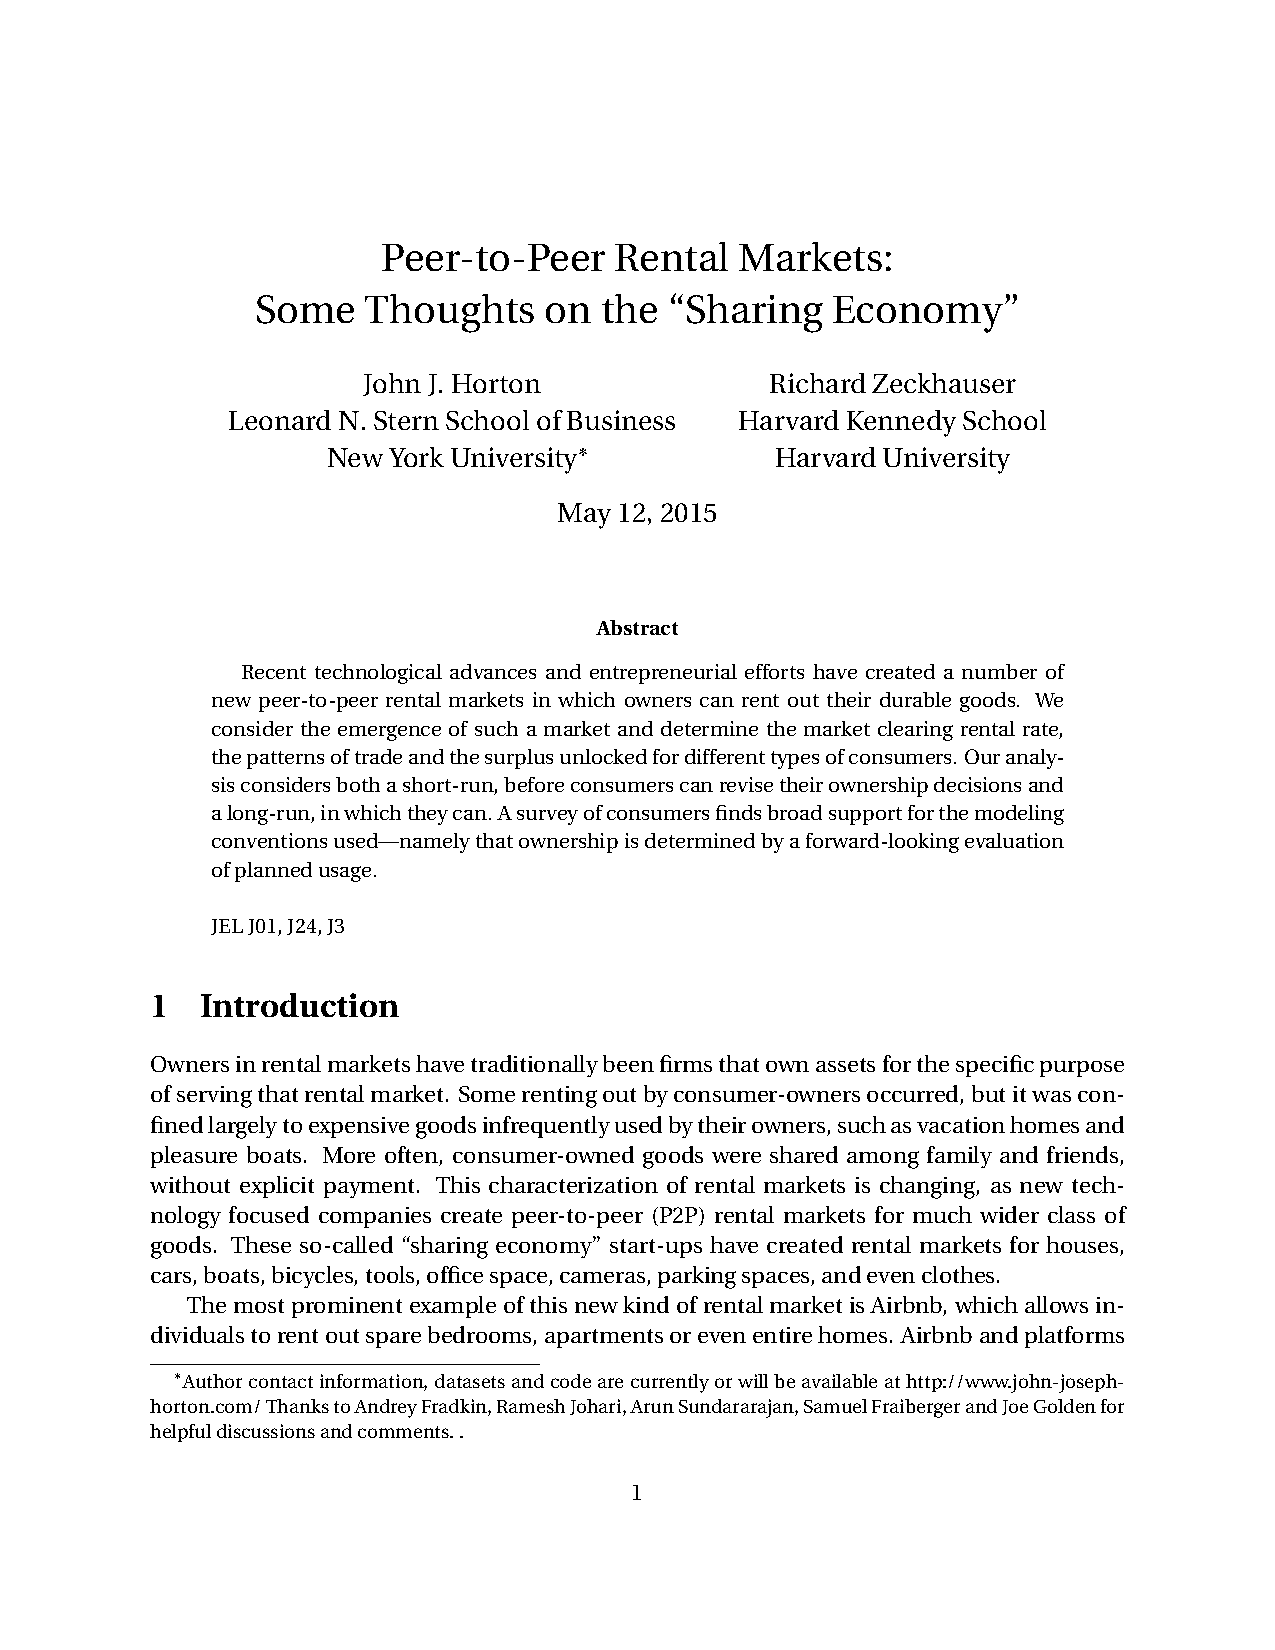
\includegraphics[width = \linewidth]{./diagrams/sharing.pdf}
{\footnotesize
\newline \emph{Notes:} This figure shows short-run market clearing in the sharing economy. 
}
\end{minipage}  
\end{figure} 

\subsection{Existence and uniqueness of a rental market} 

\begin{equation}
D(r) = \int_{\frac{c+r}{u'{0}}}^{\underline{\theta}_B} x(\theta, c +
r)\, d\theta  
\end{equation} 

\begin{equation}
D'(r) = \int_{\frac{c+r}{u'{0}}}^{\underline{\theta}_B} \frac{\partial x(\theta, c +
r)}{\partial r}\, d\theta - \frac{x\left(\frac{c+r}{u'(0)}, c + r\right)}{u'(0)} 
\end{equation} 
and since $\frac{\partial x(\theta, c+r)}{\partial r} =
\frac{1}{\theta u''(x(\theta, c + r))} < 0$ (differentiate the first
order condition), 
\begin{equation}
D'(r) = \int_{\frac{c+r}{u'{0}}}^{\underline{\theta}_B}
\frac{1}{\theta u''(x(\theta, c + r))}\, d\theta -
\frac{x\left(\frac{c+r}{u'(0)}, c + r\right)}{u'(0)}  < 0. 
\end{equation} 
A similar argument for the supply-side shows that $S'(r) > 0$. 


\paragraph{How elastic is individual demand with respect to the rental rate?} 
A consumer's intensive margin adjustment with respect to a change in the rental rate is 
\begin{equation} 
\frac{\partial x(\theta, r)}{\partial r} = \frac{1}{\theta u''(x(\theta, r))}
\end{equation} 

\paragraph{Who rents?} 

An owner that chooses to rent at the rate $r$ has 

\begin{equation}
\theta u(x(\theta, c + r)) - c x(\theta, c + r) + (1-x(\theta, c+r))r
- p - \gamma =  
\theta u(x(\theta, c)) - c x(\theta, c) - p  
\end{equation} 

\begin{equation}
\theta u(x(\theta, c + r)) - c x(\theta, c + r) + (1-x(\theta, c+r))r - \gamma =  \theta u(x(\theta, c)) - c x(\theta, c)   
\end{equation} 


At the optimum, it is still the case: 
\begin{equation}
\theta u'(x(\theta, c + r)) = c + r
\end{equation} 

\begin{equation}
\theta u'(x(\theta, c)) = c
\end{equation} 

\begin{equation}
\theta u(x(\theta, c + r)) - (c + r) x(\theta, c + r) + r - \gamma =  \theta u(x(\theta, c)) - c x(\theta, c)   
\end{equation} 

\begin{equation}
\left[ \theta u(x(\theta, c + r)) - \theta u(x(\theta, c) \right] - \left( \theta u'(x(\theta, c + r)) x(\theta, c + r) - \theta u'(x(\theta, c)) x(\theta, c) \right) = \gamma  - r     
\end{equation} 


\begin{equation}
 
\end{equation} 

\paragraph{Short-run equilibrium rental rate.} 
I define the ``short-run'' as the stock of owned goods being fixed and owned by those that would have purchased them in the absence of a sharing economy. 
Let $\underline{\theta}_R(r)$ be the first consumer that rents when the rental rate is $r$. 
The demand will be 
\begin{equation} 
D_R(r) = \int_{\underline{\theta}_R}^{\theta_B} x(\theta, r) \,dF\theta.
\end{equation} 
The supply of the good for rent is 
\begin{equation}
S_R(r) = \int_{\underline{\theta}_B}^{\bar{\theta}_B} 1 - x(\theta, r) \,dF\theta. 
\end{equation} 
Note that $\underline{\theta}_R = \frac{c + r}{u'(0)}$. 
For $\bar{\theta}_B$, renting has to be worth it, meaning that $1 - x(\theta_B, r) = \frac{\gamma}{r}$.
Note that as $r$ increases, there are two ``sources'' of supply. 
One is decreased is that higher-intensity buyers find renting more attractive (i.e., more likely to clear the $\gamma$ hurdle).
In other words, more owners are brought into the market. 
The second source of supply is economized usage by owners, who now face a higher marginal cost.
With higher $r$, demand is also reduced by two sources: economized usage, i.e., lower $x(\theta, r)$ and fewer consumers renting anything at all. 

TK---when can you differentiate with respect to an endogeneous variable? 
Of course, renters also economize in the face of higher $r$. 
All buyers and renters have the same first order condition, $\theta u(x) = c + r$, and so 
\begin{equation} 
\frac{\partial x}{\partial r} = \frac{1}{\theta u''(x)}
\end{equation}  

Figure~\ref{fig:sharing_economy} illustrates short-run market clearing. 
At a rental rate of $r$, all owners in $[\underline{\theta}_B, \bar{\theta}_B]$ will rent. 
The supply is illustrated as the yellow and green regions. 
The green region is the unused capacity when the opportunity cost of use was only $c$, i.e., before rental was possible. 
The yellow region is the capacity ``freed up'' by the owner now facing a marginal opportunity cost of $c + r$.
The dashed line at $1 - \gamma/r$ determines $\bar{\theta}_B$, which is the last owner with enough capacity (after economizing on the intensive margin) such that renting is profitable.  

\subsubsection{Long-run rental rate and product market demand} 
In the long-run, individuals can change their ownership decision. 
As both owners and renters face the same marginal opportunity cost, $c + r$, heterogeneity in consumption is a function solely of $\theta$, not of the buy/rent choice. 
As such, a consumer is deciding whether to obtain the good through rental, at a cost of $rx(\theta, r)$, 
or through purchase, at a cost of $p + \gamma + (1 - x(\theta,r))r$. 
The difference in cost from the two approaches is 
\begin{eqnarray*}
\Delta C &=& p + \gamma + (1 - x(\theta, r))r - \left(rx(\theta, r)\right) \\
         &=& p + \gamma - r, 
\end{eqnarray*} 
and so cost does not depend on $\theta$. 
As such, in equilibrium, buyer/renters are indifferent and so $p + \gamma = r$. 
The rental rate is simply the purchase price plus the fixed cost of renting. 
Note that any non-consumer that purchases a good solely to rent it out has zero profits. 

Note that in the short-run, $r$ did not depend directly on $p$, but in the long-run they are intimately linked. 
Let $r_{SR}$ be the short-run rental rate and let $r_{LR}$ be the long-run rental rate. 
Let $p_{SR}$ and $p_{LR}$ be the short- and long-run product prices, respectively.  

If $r_{SR} > p_{SR} + \gamma$, there were excess profits available to being an owner. 
As such, in the long-run, demand in the product market will go up, raising $p_{LR}$ and lowering $r_{SR}$. 
In this case, the emergence of the sharing economy causes a Jevon's paradox of increased usage. 
Produce surplus rises, but the effect on consumers is ambiguous. 
Long-run non-sharers are made strictly worse-off, as they now face a higher price in the product market. 
All consumers that would not have purchased under the pre-sharing regime are better off, as they consumer some of the good.

TK---Prior owners now sharing have an ambiguous outcome---they consumer less and pay a higher purchase price but do receive offsetting rental income.  

On the contrary, if $r_{SR} < p_{SR} + \gamma$, ownership is less attractive and in the long-run, fewer goods will be purchased, lowering prices. 
In this case, the introduction of the sharing economy is Pareto improving with respect to consumers. 
Owners that do not rent out their good get a price reduction; former non-owners get to consume some of the good. 
For owners that rent out the good, they could consumer their old $x$ (pre-sharing) at a now-lower purchase price and so are strictly better off. 

\subsection{Welfare under sharing?} 

\begin{eqnarray*}
\Delta U = \theta u(x(\theta, c+r)) - \theta u((x(\theta, c))  &=& \theta \int_0^r \frac{\partial u'(x(\theta, c + \tau))}{\partial z} \frac{\partial x}{\partial \tau} \, d\tau  \\ 
                                      &=& \theta \int_0^r \left(c + \tau\right) \frac{\partial x}{\partial \tau} \, d\tau \\   
                                      &=& \int_0^r \left(\frac{c + \tau}{u''(x(\theta, c + \tau))}\right)\,d\tau \\   
\end{eqnarray*} 
Which implies that the change in consumption utility from a small increase in $r$ is 
\begin{equation}
\frac{\partial \Delta U}{\partial r} = \frac{c + r}{u''(x(\theta, c + r))} 
\end{equation} 
When the marginal utility of more consumption is not changing very much (u'' is small), 
there is a larger consumption utility loss, since it takes a more dramatic change in consumption (i.e., a large change in $x$) to satisfy the new first order condition.  



\subsection{What determines the fixed costs of renting?} 
Technology can reduce some of the fixed costs of renting. 
The thicker the market, the easier it is to fully make use of the $1-x$, such as by finding an consumer that wants exactly $1-x$.  
Goods with predictable or easily adjustable usage patterns are more likely to be shareable. 
Owners of vacation homes can schedule their own usage easily. 

Some goods are used infrequently, but all consumers will likely want to use them at the same time. 
A back-up generator---while infrequently used---is unlikely to make a good sharing candidate, as demand spikes are likely to be correlated within an area, such as following a national disaster. 

Reset costs presumably differ by good. 
Most things---apartments, cars, clothes etc., need to be cleaned and or serviced. 
However, goods like jewelry presumably have little to no reset cost.

Goods that have a high novelty value---very steep $u(x)$ that flattens off well before $x = 1$---are particularly amenable to sharing. 
This explains why rentals or lending of videos and books are/were commonplace.  

Goods that are difficult to transport but need to be used in a different locations will be hard to share. 
However, goods that can be used on-site by different people are more likely to work. 
For example, yachts are relatively difficult to transport long distances, but there is a thriving sharing economy in boats where many want to sail on vacation: 
In the British Virgin islands charter yachts are owned by individuals. 

If $x$ is very close to $1$ for all owners, then there is little shareable supply available. 
Goods for which fractional consumption offers value will be candidates. 

If $\gamma$ is sufficiently high, then $r$ is so high that 
$\frac{c + r}{u'(0)} > \underline{\theta}_B$, there is no owner that would want to rent. 
If transaction costs are sufficiently high, then the rental rate would be too high to support a market (even though the high rental rate would tend to stimulate supply). 

\subsection{Elasticity of demand} 

For the marginal buyer in the long-run, 
\begin{equation}
\theta u(x) - c x + (1-x)r - \gamma + p = 0 
\end{equation} 
and so diferentiating with respect to $p$ gives us
\begin{equation}
u'(x)\frac{\partial x}{\partial p} 
\end{equation} 

\section{Conclusion}
In the very long-run, product differentiation could move towards making sharing more attractive. 
Individuals will purchase more durable goods to reduce the frequency of replacement. 
Goods with broad appeal will see an increase in demand compared to more idiosyncratic goods that cater to the owner's taste (similar to how re-sale value enters into some consumers decisions now). 
There will be a shift towards products that are more easily shareable. 
For example, locks on cars and houses that allow remote entry will be more appealing. 

On-going technological developments should reduce the costs of sharing. 
The Internet-of-Things will make it easier to identify goods that are not being used at a moment in time. 
It will also permit more instrumentation which in turn should facilitate contracting. 
For example, many goods might make a high resolution video, with precise time-tracked location of how they are being used, reducing concerns about moral hazard. 
As more of economic and social life are computer-mediated, platforms will use this information to verify the identify and reputation of buyers and sellers, mitigating moral hazard and adverse selection.  

Product market producers will subsidize sharing of experience goods, say by offering them at a discount to known-sharers.\footnote{GM is already doing this with RelayRides}.  

For goods for which Jevon's paradox does not hold, marketing will be re-directed towards encouraging ownership.
Barring that, advertisers will trumpet the rental stream income from a purchase and highlight the advantages of residual control rights. 
We might see more B2B rentals, particular among companies that have similar inputs but are not competitors in the product market. 
Goods with declining real prices are unattractive for sharing businesses, as the trend will be towards ownership. 

Digital goods are incredibly attractive for P2P ``rental'' but since a single owner can meet all the demand among non-owners, the rental rate is zero.
The reason is that even if the owner uses $x$, $1$ is still available to the person ``rented'' to.  
Of course, this is just piracy. 

%IP-multiplexing 

\cite{sinai2005}
\cite{ikkala2014defining}
\cite{varian2000} 
\cite{byers2013rise} 
\cite{becker1965theory} 

\bibliographystyle{aer}
\bibliography{sharing.bib}

\end{document} 


%Some goods are easy to make a consumption plan for---rental homes, high-end camera equipment. 
% While it makes sense to think of consumers making an extensive margin decision---buy or not buy---their individual decision, at least for some goods, is based on a solution to another optimization problem. 
% When considering a purchase, individuals are deciding ``how much am I going to use this?'' 
% This decision has to be made for nearly every consequential purchase. 
% Once a durable good is purchased, the cost of using---less depreciation---is the opportunity cost of doing something else. 
% Once purchased, a good is used up until the point that its declining marginal utility equals only the opportunity cost. 
% This is a different decision than one makes if using a rental, where the marginal cost is both the opportunity cost and the rental rate.

% When the capital costs are very high but usage by owners is relatively low, it is more likely that there are large numbers of would-be consumers and the excess capacity to satisfy them.  
% Goods being offered my a monopolist are likely to be below the  
% Most people spent only about two minutes a day brushing their teeth, giving them 4,598 minutes they could rent out their toothbrush.  
% But reset costs are likely to be high, people want to brush around the same times each day and the price of a toothbrush is so low that anyone who brushes their teeth finds it more convenient to own. 

% % Idea: time use survey 
% Owning a good and renting it out generates costs. 
% Some of these are recognizable transaction costs, such as finding a renter and coming to terms. 
% There is also the cost of writing contracts and monitoring compliance, purchasing insurance, dealing with moral hazard and adverse selection.\footnote{High-end car company had its entire fleet of fancy cars stolen.} 

% The main effect of IT when paired with for-profit platforms are reductions in the costs of renting. 
% The platforms aggregate demand and expose where supply resides, reducing search costs. 
% They have standardize contracts. 
% They measure usage and handle payments. 
% They invest in tools to reduce information asymmetries and moral hazard. 

% % How much time was spent with a good  
% % How much that good or service costs

% What IT enables: 
% - aggregate demand 
% - expose where the supply resides 
% - overcome informational problems (information asymmetries and moral
% hazard) 
% - payment timing issues (the escrow problem) 
% - Adding complexity of moral hazard. 

% Similar to P2P electronic commerce in many respects.  Uber and Airbnb are the most prominent examples. 
% The sharing economy raises several economic questions whose answer is not intuitively obvious. 
% On the one hand, if individuals can rent infrequently used property to each other, then it seems plausible that fewer of those things are actually needed. 
% For example, it is easy to imagine one suburban neighborhood sharing a single drill, whereas before, multiple households would have purchased one. 
% Of course, rental markets are not new. 
 % On the other hand, when individuals can share durable goods among themselves the greater intensity of use may actually increase demand: 
% this ``rebound effect'' or Jevons paradox seems possible. 
% Another question is who participates in the sharing economy: 
% heavy users of some durable good are likely to purchase rather than rent, but they are also unlikely to rent the item out as they are unlikely to have much spare capacity to rent. 
% Light users do have more capacity, but they are potentially the ones that get the least utility from the good anyway. 
